\documentclass[12pt, letterpaper]{article}
\usepackage{graphicx}

\usepackage{tikz}
\usetikzlibrary{automata, positioning, arrows}

\tikzset{
    ->, % makes the edges directed
    >=stealth', % makes the arrow heads bold
    node distance=3cm, % specifies the minimum distance between two nodes. Change if necessary.
    every state/.style={thick, fill=gray!10}, % sets the properties for each ’state’ node
    initial text=$ $, % sets the text that appears on the start arrow
}

\title{Leipzig Gophers 43}
\author{Leipzig Gophers}
\date{May 2024}

\begin{document}
\begin{figure}[ht] % ’ht’ tells LaTeX to place the figure ’here’ or at the top of the page
    \centering % centers the figure
    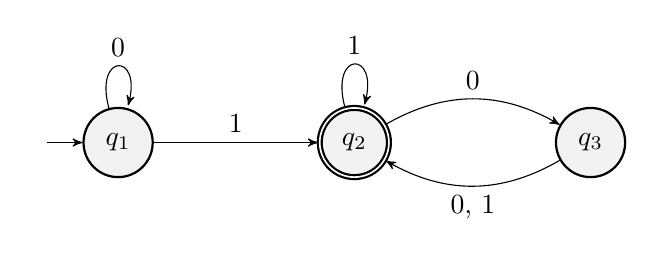
\begin{tikzpicture}
        % tikz code goes here
            \node[state, initial] (q1) {$q_1$};
            \node[state, accepting, right of=q1] (q2) {$q_2$};
            \node[state, right of=q2] (q3) {$q_3$};
            \draw (q1) edge[loop above] node{0} (q1)
            (q1) edge[above] node{1} (q2)
            (q2) edge[loop above] node{1} (q2)
            (q2) edge[bend left, above] node{0} (q3)
            (q3) edge[bend left, below] node{0, 1} (q2);
    \end{tikzpicture}
    \caption{A finite state machine corresponding to $(0^*)1(1^*)(00|01)^*$}
    \label{fig:my_label}
\end{figure}
\end{document}

